\documentclass{book}
\usepackage[english]{babel}
\usepackage[letterpaper,top=2cm,bottom=2cm,left=3cm,right=3cm,marginparwidth=1.75cm]{geometry}

\usepackage{amsmath}
\usepackage{graphicx}
\usepackage{float}
\usepackage{chemformula}
\usepackage{subfig}


\usepackage[export]{adjustbox}

\usepackage{biblatex}
\addbibresource{bibly.bib}

\title{Molecular Pharmacology Notes}
\author{Elisa Pettinà}

\begin{document}
\maketitle

\chapter{Pharmacokinetics}
\section{{What is a drug?}}
\textbf{A drug is a chemical that interacts with proteins in the body to affect a physiological function}.
Once these chemicals are absorbed into the systemic circulation they bind with certain proteins and this changes the functioning of the cell slightly. 
For example, anticancer drugs bind to proteins on the surface of cancer cells this stimulates the cells to die. 
In this case cell death is the physiological action of the drug.
\\
No drugs are specific to interacting with just one type of cell or one type of protein
and this is what causes \textbf{side effects}. 
Again using an anticancer drug as an example, the medication works by binding to very rapidly dividing cells, such as cancer cells, however hair cells are also rapidly dividing and that is why one of the side effects of anticancer drugs is hair loss.
\\
Drugs can be generally divided into two main categories: \textbf{agonist}, that stimulate a response and \textbf{antagonist}, that inhibit a response.

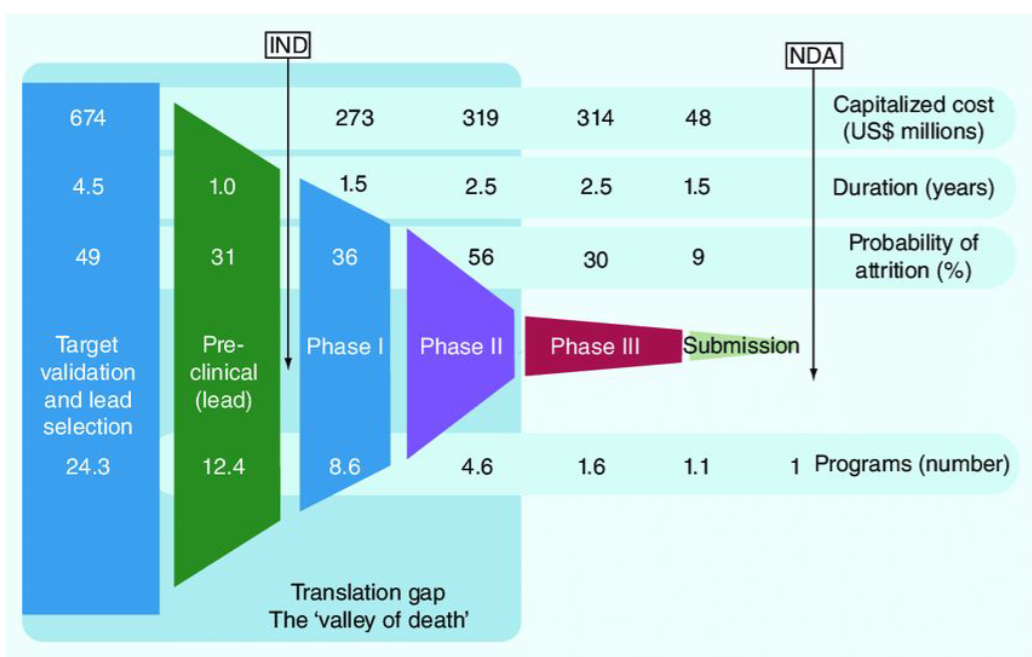
\includegraphics[width=0.7\textwidth, center]{images/image.png}

Developing and testing drugs is a very expensive business!
Many parameters regarding pharmacokinetics and pharmacodynamycs need to be taken studied and fit into strict boundaries for the drug to be accepted.

\section{Pharmacokinetics}
Pharmacokinetics (PK) is the study of how the body interacts with administered substances for
the entire duration of exposure.
In other words, \textbf{what the body does to the drug(s)}!
\\
For a chemical compound to become a marketable drug, it must have favourable properties in addition to \textbf{efficacy} (its therapeutic effect) and \textbf{safety}. 
These properties are summarised in the acronym ADME, which refers to \textbf{absorption}, \textbf{distribution}, \textbf{metabolism} and \textbf{excretion}.

\begin{itemize}
    \item Absorption: a compound's ability to pass through barriers such as the intestinal lining, the nasal lining, the lungs or the skin.
    \item Distribution: how the compound is distributed around the body and its propensity to accumulate in certain tissues and organs.
    \item Metabolism: how the body breaks down the compound, normally by the liver. The key issues are drug-drug interactions and the effects of the metabolites (the new chemicals created as a result of metabolism).
    \item Excretion: the rate and process through which the compund exits the body.
\end{itemize}

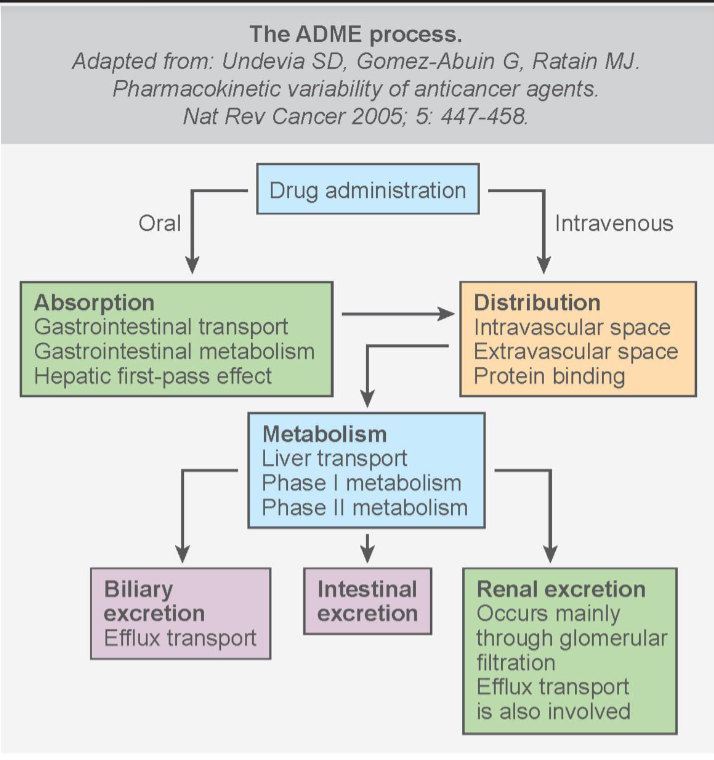
\includegraphics[width=0.6\textwidth, center]{images/image_1.png}

Often we refer also to \textbf{AADME}, including also \textbf{administration}, which also greatly influences the PK properties of drugs and drug concentration in plasma.

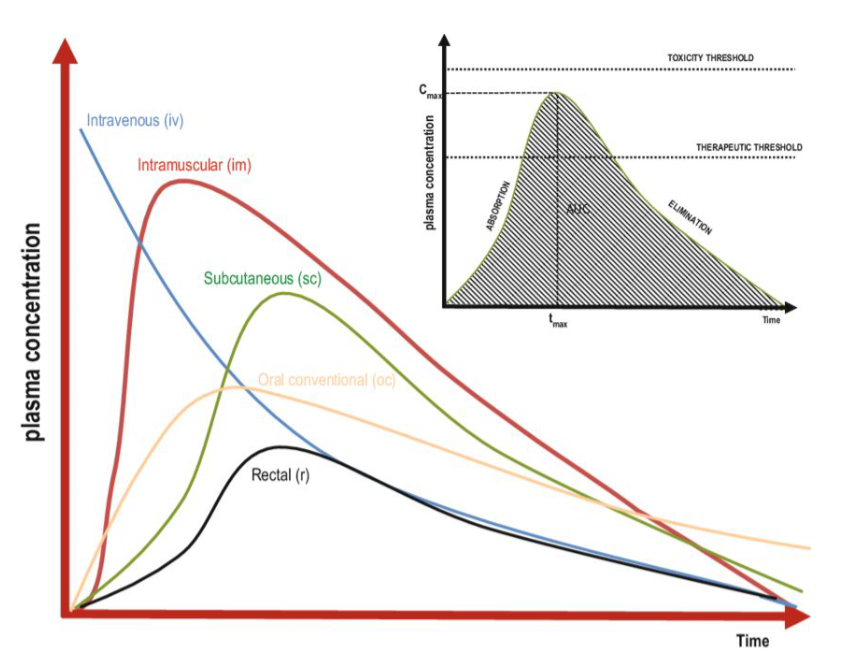
\includegraphics[width=0.6\textwidth, center]{images/image2.png}


\subsection{Absorption}
\textbf{Absorption is the process of a drug moving from its site of delivery into the bloodstream}.
\\
Absorption is the process of delivering a drug into the bloodstream. 
Absorption can be accomplished by administering the drug in a variety of different ways (e.g. orally, rectally, intramuscularly, subcutaneously, inhalation, topically, etc.). 
Note, that if a drug is administered intravenously (placed directly into the bloodstream), the need for absorption is bypassed entirely.
\\
However, the plasmatic membrane cannot be passed freely.
Gases ($CO_2$, $N_2$, $O_2$, anaesthetic), small uncharged polar molecules (ethanol, urea, water) can pass easily. Inversely, large uncharged polar molecules (sugar), ions and charged polar molecules (amino acids, ATP, proteins, nucleic acids) cannot.
\\
\\
The need for drug molecules to cross lipid bilayers in passing from one body compartment to another requires that the structure has properties that impart solubility in both a hydrophobic medium and water. 
Each part of a drug molecule contributes hydrophobic or hydrophilic properties to the molecule as a whole and that contribution is known as the \textbf{Hansch partition coefficient} of the
group.

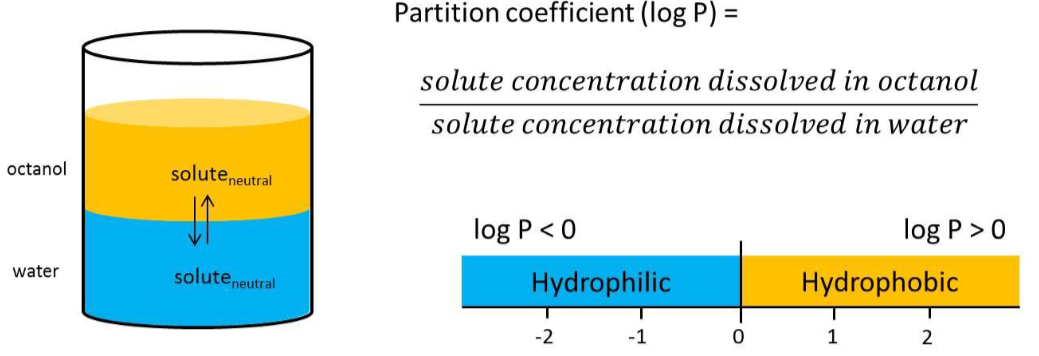
\includegraphics[width=0.6\textwidth, center]{images/image3.png}

\subsection{Distribution}
\textbf{Drug distribution is the process of delivering a drug from the bloodstream to
the body}.
The process of transferring a drug from the bloodstream to tissues is referred to as distribution. 
The same principles that govern drug absorption (e.g. ionization of a drug, lipophilicity of a drug, size of a drug, pH of the environment, etc.) also govern the rate and extent that a drug will distribute to various tissues in the body. 
In addition to that, there are additional factors at play, particularly non-specific binding to proteins.

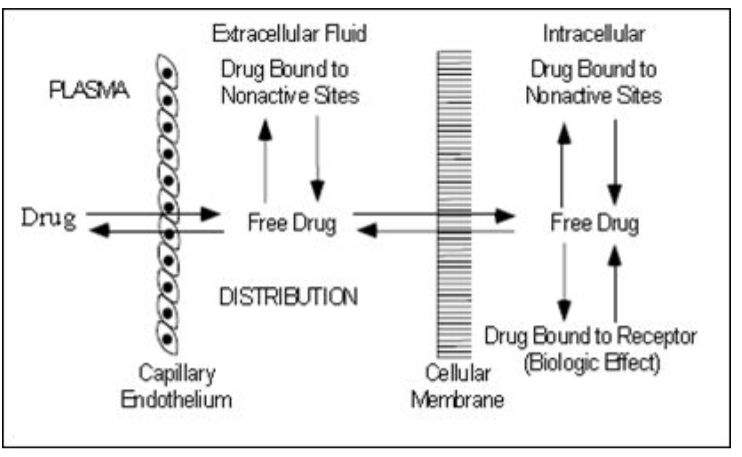
\includegraphics[width=0.6\textwidth, center]{images/image4.png}

\subsubsection{Volume of distribution}
The concept of “apparent volume of distribution” is a concept that seeks to predict how
extensively a drug is distributed throughout the body. 
The apparent volume of distribution, $Vd$, is mathematically calculated by dividing the dose that is administered ($mg$) by the plasma concentration C ($mg/L$).

\begin{equation*}
    Vd = \frac{Dose}{C}
\end{equation*}

Based on the above equation:

\begin{itemize}
    \item A drug with a high $Vd$ has a propensity to leave the plasma and enter the extravascular compartments of the body, meaning that a higher dose of a drug is required to achieve a given plasma concentration. (High $Vd$ $\rightarrow$ More distribution to other tissue)
    \item Conversely, a drug with a low $Vd$ has a propensity to remain in the plasma meaning a lower dose of a drug is required to achieve a given plasma concentration. (Low $Vd$ $\rightarrow$ Less distribution to other tissue)

\end{itemize}

Another way to think about $Vd$ is that $Vd$ is equal to the amount of space that a drug
must fill up such that a given dose of a drug will achieve a specific plasma concentration. 
There is an assumption here; that is, calculation of the apparent $Vd$ presumes that the drug concentration is the same everywhere throughout the body.
We know though that this is not true since most drugs are not uniformly distributed.
More on this on the NIH website\cite{NIH}.

\begin{figure}
    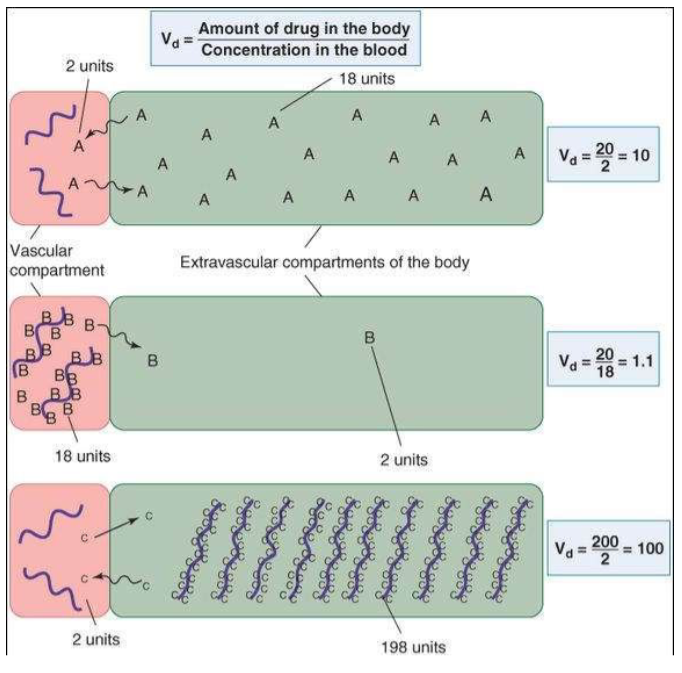
\includegraphics[width=0.6\textwidth, center]{images/image5.png}
    \caption{Drug A diffuses freely between the two compartments. Drug B binds avidly to plasma proteins and is retained in the plasma compartment (low $Vd$). Drug C binds avidly to molecules in peripheral tissues. Low concentration in blood, thus high $Vd$ and higher total dose required to achieve measurable plasma centration.}
\end{figure}

\textbf{Binding to plasma proteins} highly influences the volume of distribution and in general, drug efficacy, distribution, and disposition. 
Serum albumin displays an extraordinary ligand binding capacity, and a-1-Acid glycoprotein is the main carrier for basic and neutral drugs.
High- and low-density lipoproteins play a limited role in drug binding.
\\
\\
Drug distribution is also influenced by physio-anatomical features.
For example, brain capillaries are different from general capillaries in the body, forming the \textbf{blood-brain-barrier} (BBB).
The BBB is composed of specialized endothelial cells, pericytes, a capillary basement membrane, and astrocyte end-feet, all working together to protect the brain from harmful substances while allowing essential nutrients and molecules to enter. 
The BBB's selectivity is crucial for maintaining a stable and optimal environment for brain function. 
The placenta is also a barrier (placental barrier) to be taken into account.

\subsection{Metabolism}
The primary objective of drug metabolism is to facilitate a drug's excretion by increasing its
water solubility (hydrophilicity). 
The involved chemical modifications incidentally decrease or increase a drug's pharmacological activity and/or half-life.
The principal organs of drug metabolism are the liver and (for orally taken drugs) the small intestine. 
Drugs completely inactivated during the first-pass through these organs must be given parenterally, similarly to poorly absorbed drugs.

\begin{figure}
    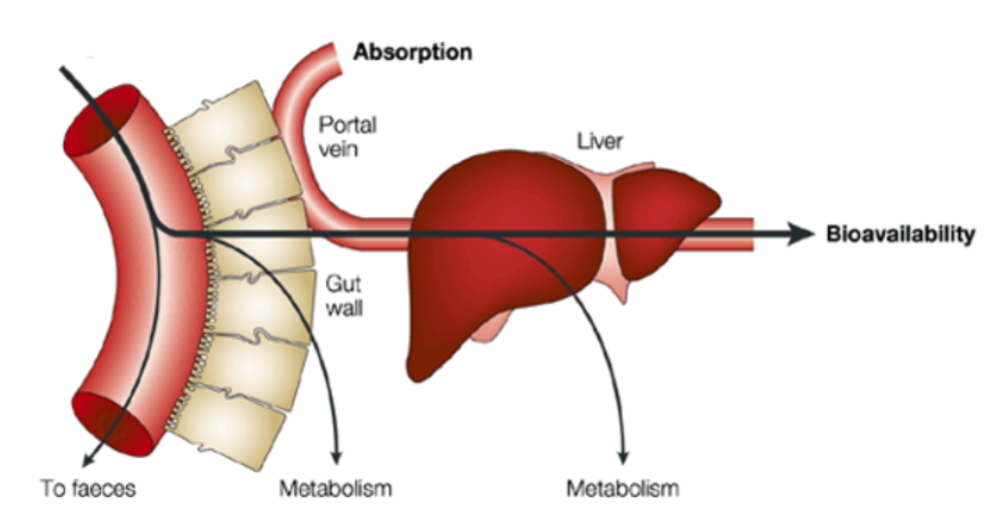
\includegraphics[width=0.6\textwidth, center]{images/image6.png}
    \caption{\textbf{First pass effect}- The large reduction in concentration of an orally absorbed drug due to passage of the drug through the liver.  Some drug will be lost during absorption from the intestine and more from metabolism in the liver. Remember, the liver sees many things as potential toxins and tries to detoxify them. Drugs are included in that list of things that the liver tries to remove. \textbf{Bioavailability}– the fraction of the drug that escapes the liver and reaches the systemic circulation due to the first pass effect.  If a drug is given intravenously, it is considered to have 100\% bioavailability since it is all in the blood stream. The same drug given orally will have less bioavailability since some is never absorbed (stays in the gut and ends up in the feces) or is modified by the liver before it hits the vascular system.}
\end{figure}

\subsubsection{Cytochromes P450 and transporters}
CYPs are hemeproteins used extensively by the liver to metabolize drugs. 
The types and amounts of CYPs vary by species, sex and genetic makeup. 
The main families of CYP450 enzymes involved in drug metabolism are the monooxygenases of the CYP1, CYP2 and CYP3 families.
Changes in CYPs result in different levels of drug effectiveness and toxicity. 
Differences in cyp450 is responsible for the unique responses of horses and cats to certain drugs.

Drugs can interact with CYPs in 3 different ways:

\begin{itemize}
    \item Drugs may just be metabolized by the CYPs. Generally this makes drugs less available to the animal as it leads to faster excretion.
    \item Drugs may inhibit CYP activity. Erythromycin and omeprazole inhibit CYP activity. This prevents the CYPs from metabolizing other drugs being administered to the animal, resulting in abnormally high levels of the unmetabolized drugs.
    \item Drugs may induce CYP activity. Phenytoin, phenobarbital, griseofulvin and rifampin are CYP inducers. When they are present, the CYPs metabolize other drugs at a much higher rate, resulting in low working levels of those drugs.
\end{itemize}

However, drug metabolism does not happen only in the liver! 
\textbf{P-glycoprotein 1} is important protein of the cell membrane that pumps many foreign substances out of cells.
P-gp is extensively distributed and expressed in the intestinal epithelium where it pumps xenobiotics back into the intestinal lumen, in liver cells where it pumps them into bile ducts, in the cells of the proximal tubule of the kidney where it pumps them into urinary filtrate (in the proximal tubule), and in the capillary endothelial cells composing the blood–brain barrier and blood–testis barrier, where it pumps them back into the capillaries.
\\
\\
Another important family of cell transporters are the \textbf{ABC-type ATPases}.
Of this family we also find \textbf{P-glycoprotein} (\textbf{Pgp}), also known as multidrug resistance protein 1 (MDR1) or ATP-binding cassette sub-family B member 1 (ABCB1), which is a transmembrane protein that acts as an efflux pump, transporting various substances out of cells.
It plays a role in drug resistance in cancer and also has physiological functions in various tissues like the intestines, liver, and brain. 

\subsubsection{Other factors influencing drug metabolism}
There's a plethora of factors that contribute in differences in drug metabolism, e.e. sex, age, polymorphism, diseases\dots.
Another important aspect to consider is drug interactions.
The interactions can happen with other drugs, supplements or medical conditions.
For example, injesting grapefruit blocks CYP3A4 enzyme in enterocytes and in the liver, which metabolizes the drug felodipine.
Usually CYP3A4 metabolizes the drug to the 15\%, but grapefruit increases bioavailability to 45\%

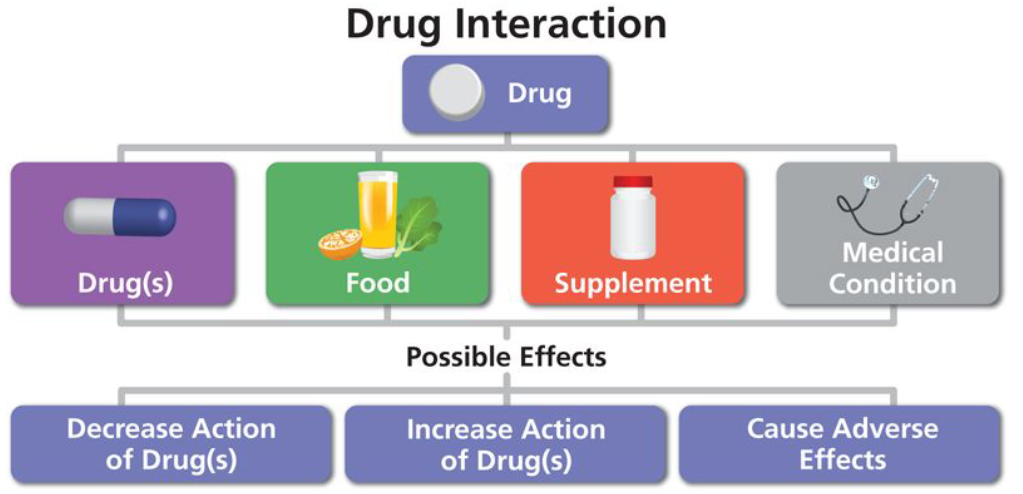
\includegraphics[width=0.6\textwidth, center]{images/image7.png}


\subsection{Excretion}
\textbf{Excretion is the removal of drugs and their metabolites from the body.}
The kidney is the principal drug-excreting organ. 
All renally excreted drugs reach urine via glomerular filtration. Many drugs additionally are secreted into the proximal tubule through the opportunistic (molecular similarity-based) use of organic cation and anion transporters. 
Lipophilic drugs are additionally secreted into the proximal tubule via passive diffusion, as they can easily cross the membranes of nephron cells.
\\
\\
Excretion can also happen by the bile (and thereby with stool), sweat, exhaled air, saliva, and breast milk, but they play a much smaller role compared to urine.
An exception is the excretion of volatile anesthetics with exhaled air.

\begin{figure}

    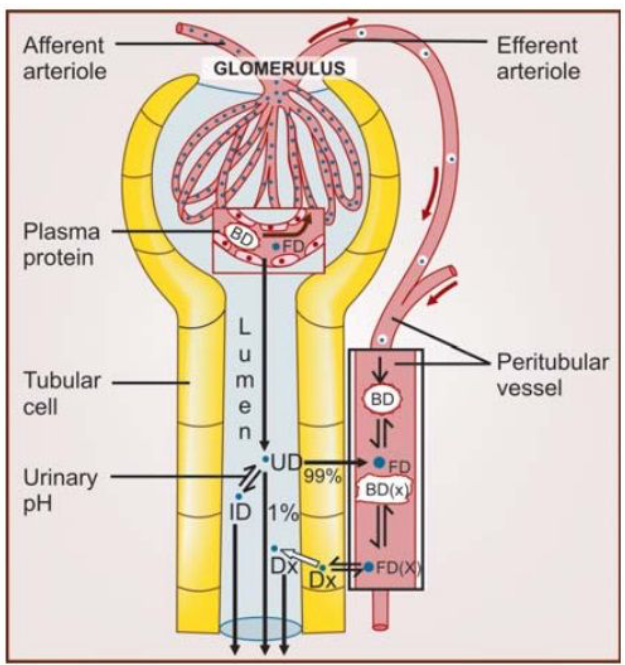
\includegraphics[width=0.4\textwidth, center]{images/image8.png}
    \caption{Schematic depiction of glomerular filtration, tubular reabsorption and tubular secretion of drugs. FD - free drugs; BD - bound drug; UD - unionized drug; ID - ionized drug; Dx - actively secreted organic acid (or base) drug.}
    
\end{figure}

\subsubsection{Drug Clearance}

Drug clearance (body clearance, total body clearance, or $Cl_T$) is a pharmacokinetic term for describing drug elimination from the body without identifying the mechanism of the process.
Clearance is calculated based on plasma drug concentration data.

\begin{equation*}
    Cl_T = \frac{\text{elimination rate}}{ \text{plasma concentration} (C_p)}
\end{equation*}
\begin{equation*}
    Cl_T = \frac{dD_E / dt}{C_p} = \frac{\mu g / min}{\mu g /ml} = ml/min
\end{equation*}

Where $D_E$ is the amount of drug eliminated and $dD_E / dt$ is the rate of elimination.
Clearance relates to volume of distribution through the following equation:

\begin{equation*}
    Cl_T = \frac{kC_pV_D}{C_p} = k V_D
\end{equation*}

Clearance is the product of $V_D$ and $k$, both of which are constant.
As the plasma drug concentration decreases during elimination, the rate of drug elimination, $dD_E / dt$, decreases accordinlgy, but clearance remains constant.
Clearance is constant as long as the rate of drug elimination is a first-order process.

\begin{figure}
    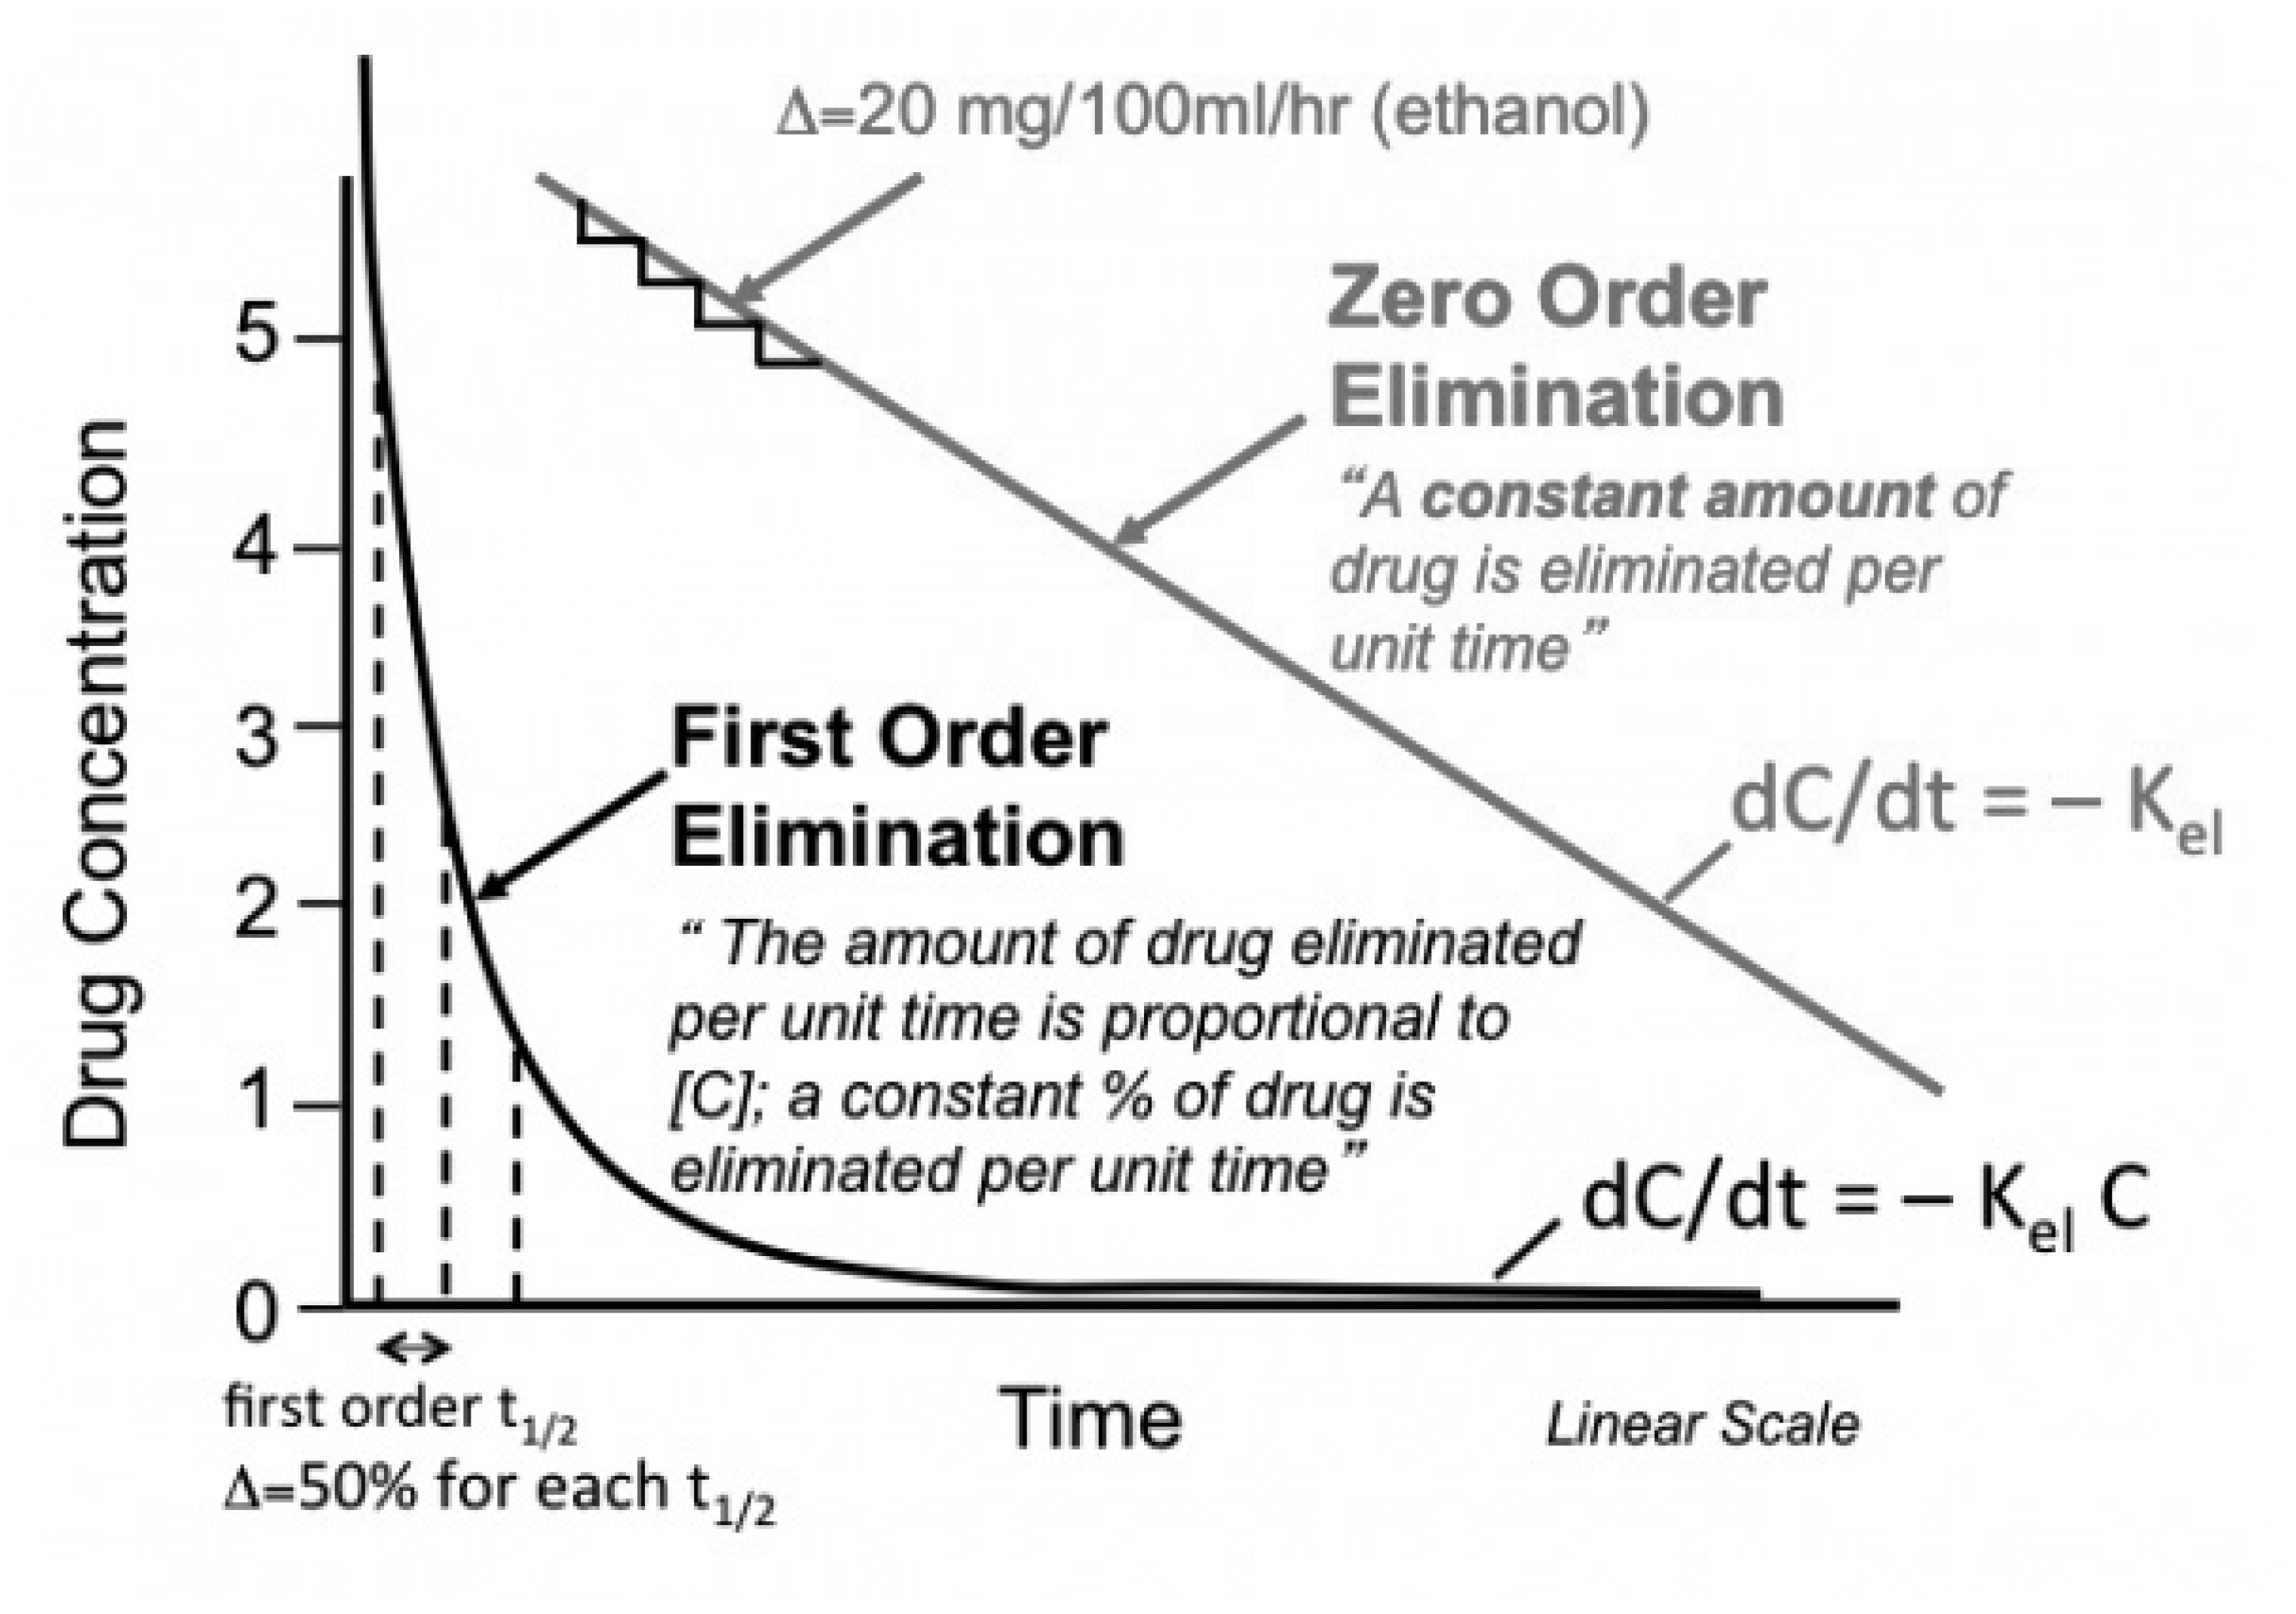
\includegraphics[width=0.6\textwidth, center]{images/image9.png}

    \caption{In medical science, the term half-life typically refers to the elimination half-life. The elimination half-life is defined as the time required for the concentration of a specific substance, typically a drug, to decrease to half of its initial amount in the body. Although different drugs have varying half-lives, they all share a common principle—after one half-life, 50\% of the initial drug amount is removed from the body. Most clinically relevant drugs follow first-order pharmacokinetics, meaning their drug-elimination rates are directly proportional to plasma concentrations.[1] In contrast, a few drugs follow zero-order elimination, in which the drug amount decreases by a constant amount over time, regardless of initial concentration, for example, ethanol. For more info check \cite{NIH_halflife}.}
\end{figure}

\subsubsection{Free Drug is the Active Fraction}

A basic tenet of clinical pharmacology is that only unbound (free) drug molecules can interact with target receptors that are present on cell membrane or with enzymes that are located inside the cell, and therefore the intensity and duration of drug action are mediated via the time course of unbound drug concentrations at the site of action. 
With few exceptions, most drug target receptors or enzymes are located outside of the blood circulation in the target tissues. 
Although unbound drug concentrations in blood can be readily measured, direct assessment of unbound drug concentration at the action site in target tissues is seldom possible due to inaccessibility of the action sites.
\\
For this reason, the unbound drug concentration in blood (plasma) is often used to establish pharmacokinetics‐pharmacodynamics (PK‐PD) relationship by applying the so‐called \textbf{free drug hypothesis}. 
The hypothesis assumes that the unbound drug concentration in blood is the same as that in the site of action at steady state.
From literature, the free drug hypothesis appears valid for many drugs. 
The unbound concentrations of drugs in peripheral tissues and brain are quantitatively similar to those in plasma.
However, the hypothesis is not applicable for some drugs. For examples, the unbound concentrations of morphine, gabapentin, and atenolol in the brain are significantly lower than those in plasma.
\\
Over the years, with the progress of molecular biology, it has become evident that efflux drug transporters (such as P‐gp, BCRP, and MRPs) play an important role not only in drug excretion but also in tissue distribution (drug transport), particularly for brain uptake.
For drugs that are substrates of efflux transporters, at steady state, the unbound drug concentrations in tissues are expected to be lower than unbound drug concentrations in plasma, when efflux transporters are involved in tissue distribution. 
Based on the involvement of efflux transporters, drugs can generally be categorized into two classes: drugs that are not substrates of efflux transporters (Class I) and drugs that are substrates of efflux transporters (Class II). 
It is expected that the free drug hypothesis will not be valid for drugs that are substrates of efflux transporters. 
Conceivably, the free drug hypothesis is also not applicable for drugs that are substrates of influx transporters. 
Unbound drug concentration in tissues is expected to be higher for influx transporter drugs than that in plasma.

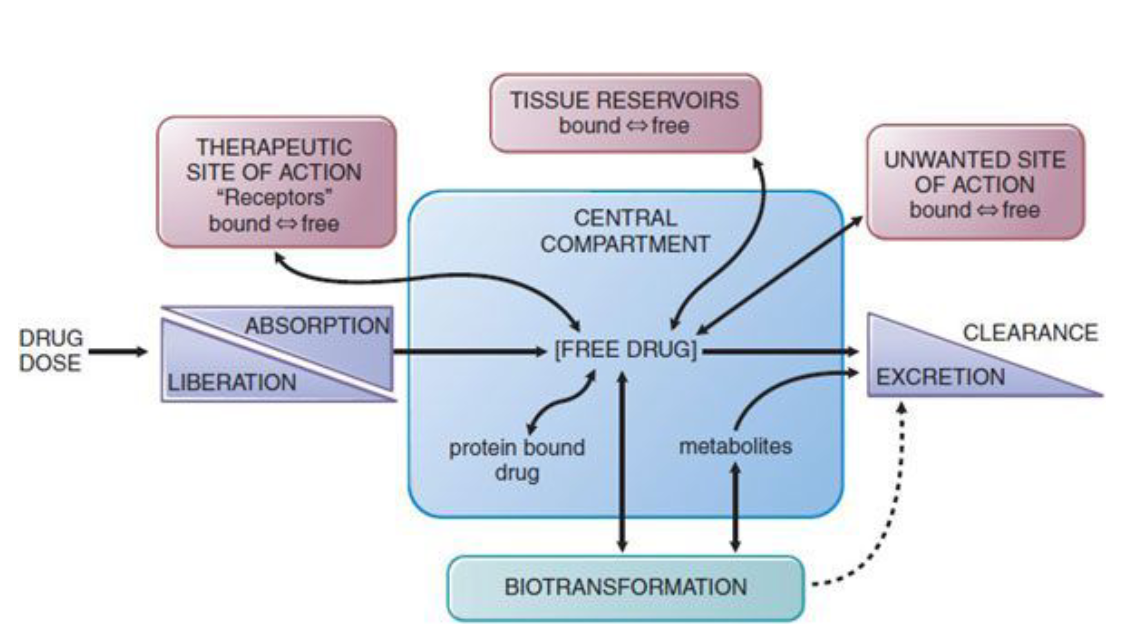
\includegraphics[width=0.8\textwidth, center]{images/image10.png}

\subsection{General PK considerations}
Other basic PK concepts are :
\begin{itemize}
    \item MEC: minimum effective concentration
    \item MTC: minimum toxic concentration
\end{itemize}

Everything under MEC is considered "sub therapeutic level", everything above MTC is considered at "toxic level'.
The first intersection of drug concentratoin with MEC is called "onset time", and the second intersection "termination of action".

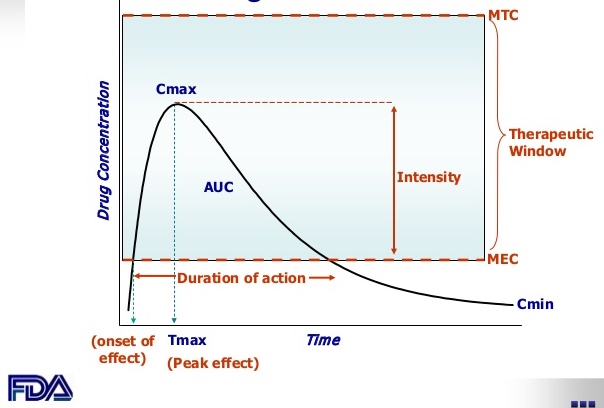
\includegraphics[width=0.7\textwidth, center]{images/image11.png}


\chapter{Pharmacodynamics}


pharmacodynamicsis the other branch, together with pharmacokinetics, of pharmacology.

In particular, pharmacodynamics is the study of \textbf{how a drug affects an organism}, whereas pharmacokinetics is the study of how the organism affects the drug. 
Both together influence dosing, benefit, and adverse effects. 

Pharmacodynamics places particular emphasis on dose–response relationships, that is, the relationships between drug concentration and effect.
One dominant example is drug-receptor interactions as modeled by \ch{L + R <=> LR}, where $L$, $R$, and $LR$ represent ligand (drug), receptor, and ligand-receptor complex concentrations, respectively. 

\section{Drug Targets}
Drug targets can be any structure in the cell and often they are cell receptors.

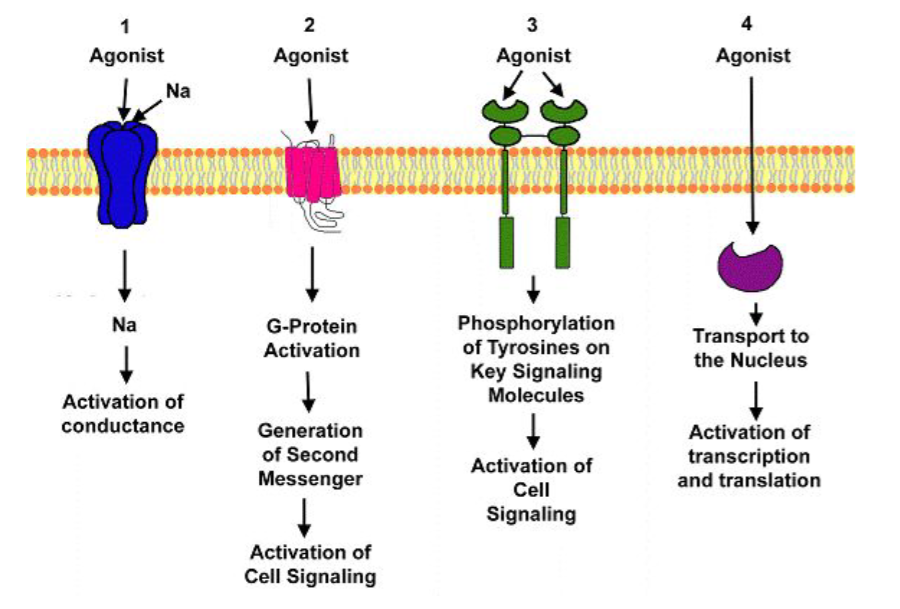
\includegraphics[width=0.7\textwidth, center]{images/image12.png}

\section{Dose Response Curve}
The pharmacological effect of a drug depends on its concentration at the site of action, which in turn is determined by the dose of the drug administerd.
Such a relationship is called the \textbf{D-R}.
\\
The idea is that the extent to which the desired response alters as the dose changes.
The dose is plotted on the horizontal axis and the response on the vertical axis.

\subsection{Graded dose-response graphs}
Graded dose-response curves are graphical representations of the relationship between the dose of the drug and the effect it achieves. 
More specifically, the concentration of the drug is used, rather than the actual dose.
\\
They are also usually plotted on a logarithmic scale of concentration which stretches the lower end of the dose range, to inflate the useful (20\%-80\%) response range where dose-effect relationship is linear, and to compress the clinically uninteresting high and low dose ranges.

\begin{figure}
    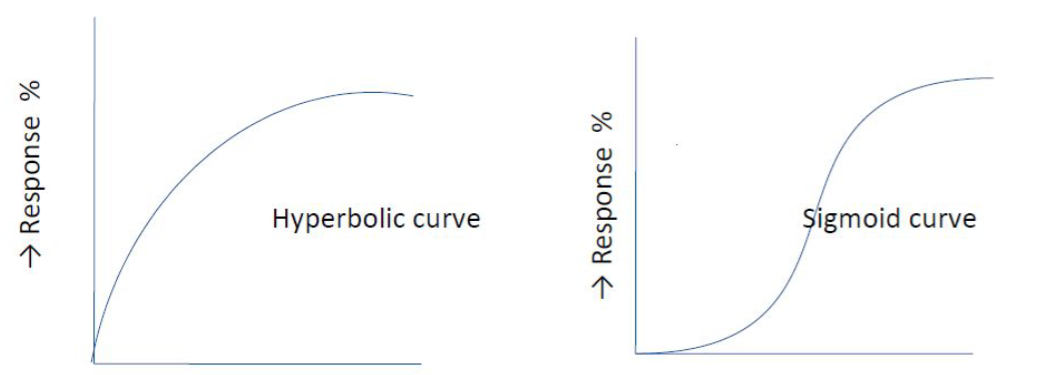
\includegraphics[width=0.7\textwidth, center]{images/image13.png}
    \caption{Difference in plotting between dose and logDose}
\end{figure}

Graded dose-response curves provide insights to these properties:

\begin{itemize}
    \item Affinity ($K_d$): the tendency of a drug to bind to the receptor, or the extent to which a drug can produce a response when all available receptors or binding sites are occupied. 
    \item Efficacy: the capacity of a s drug -receptor complex to elicit response.
    \item Potency:  the uantity of a drug required to produce the desidered response (more potent drugs producce effects at lower concentratoins). Potency refers to the concentration ($EC_{50}$) or dose ($ED_{50}$) of a drug. The potency of a drug depends on the affinity ($K_d$) and in part on the efficacy with which drug-receptor interaction is coupled to response.
\end{itemize}

\begin{figure}[H]
    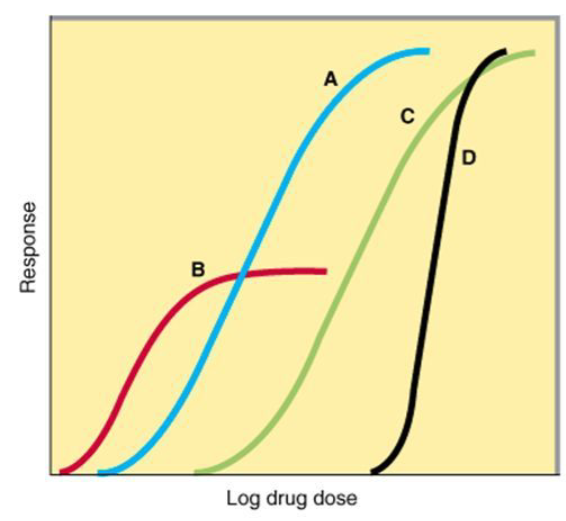
\includegraphics[width=0.35\textwidth, center]{images/image14.png}
    \caption{Graded dose-response curves for drugs, illustrating different pharmacological potencies and different maximal efficacies. Potency: $B>A>C>D$, Efficacy: all same except for B (lowest).}
\end{figure}


\subsection{Therapeutic Index (Therapeutic Window)}
\begin{quotation}
    \textit{Solely the dose determines that a thing is not a poison}
\end{quotation}

Vitamin A, essential for sustaining life, can be lethal if taken in very doses, and botulin toxin can not cause damages (and even be beneficial) at very low doses.
\\
The therapeutic index is a ratio that compares the blood concentration at which a drug becomes toxic and the concentration at which the drug is effective. 
The larger the therapeutic index (TI), the safer the drug is. If the TI is small (the difference between the two concentrations is very small), the drug must be dosed carefully and the person receiving the drug should be monitored closely for any signs of drug toxicity.

\begin{equation*}
    TI = \frac{TD_{50}}{ED_{50}}
\end{equation*}

However, nowadays the term "therapeutic window" or "therapeutic range" is preferred, which is determined after all the studies on the drug of interest.
Importantly, this window is not fixed, rather it depends on the age and other physiological characteristics.

\begin{figure}[H]
    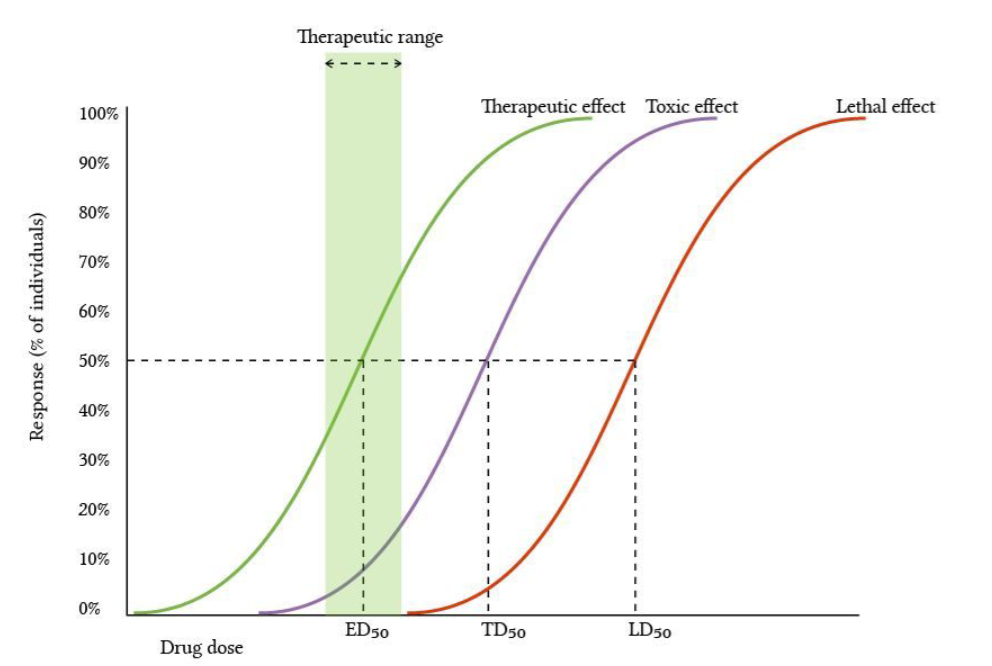
\includegraphics[width=0.7\textwidth, center]{images/image15.png}
    \caption{}
\end{figure}

\section{Agonists and Antagonists}

Basically any receptor can be subjected to agonist and antagonist drug.

\begin{itemize}
    \item Agonists: drugs that occupy receptors and activate them.
    \item Antagonists: drugs that occupy receptors but do not activate them. They also can lessen the activation by agonists.
\end{itemize}

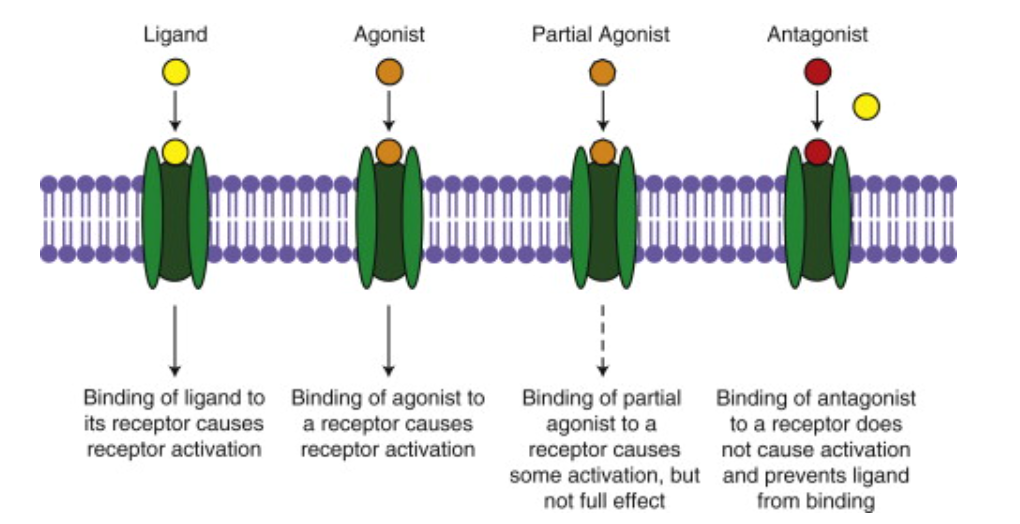
\includegraphics[width=0.7\textwidth, center]{images/image16.png}

\subsection{Agonists}
Agonism describes the process of binding of a drug to its specific receptor, activate it and produce some molecular and cellular response.
\\
In other words, agonists are the chemical substances, or drugs, that can interact (combine) with a receptor (affinity) and thereby initiate a cellular reaction (efficacy).
E.g. adrenaline in cardiac arrest stimulates $\beta_1$ receptor - increasing the force of contraction and heart rate.
Their efficacy is $1$ (or $100\%$).

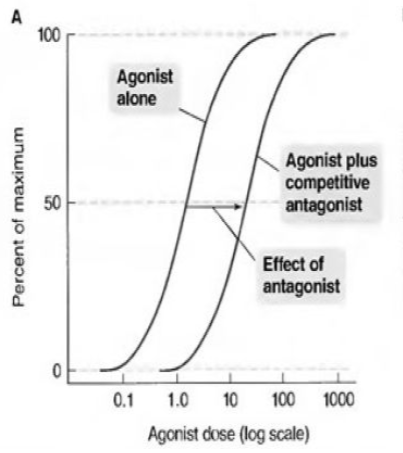
\includegraphics[width=0.35\textwidth, center]{images/image17.png}

A \textbf{partial agonist} binds to its receptor but produces a smaller effect than a full agonist.
Their effiacy is between $0-1$.

\begin{figure}[H]
    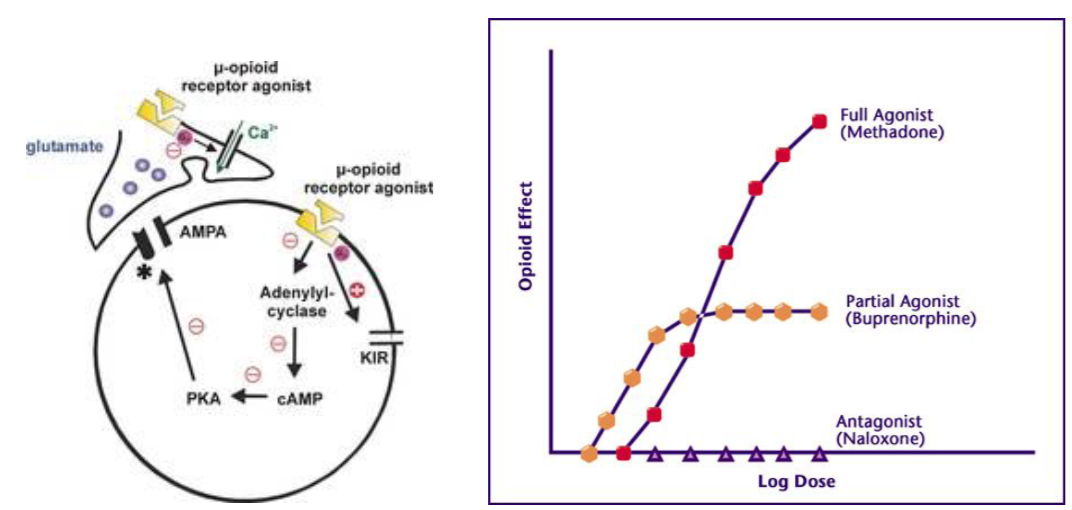
\includegraphics[width=0.8\textwidth, center]{images/image18.png}
    \caption{Pain killers can be full agonists, partial agonists or antagonists. Nalozone is an opioid antagonist medication used to reverse or reduce the effects of opioids, particularly in cases of overdose. It works by blocking the effects of opioids on the body, restoring breathing if it has been depressed by opioids.}
\end{figure}

\subsubsection{Inverse Agonist}
Inverse agonists bin\d to a receptor and produce the opposite effect.
In this case, the efficacy is $-1$.
Examples are benzodiazepines, that produce CNS depression, while $\beta$ carbolines produce excitation, anxiety and convulsion.

\begin{figure}[H]
    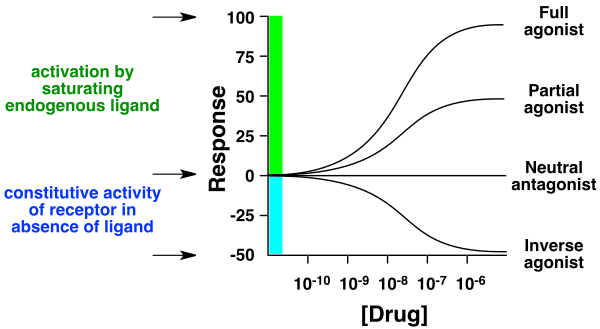
\includegraphics[width=0.6\textwidth, center]{images/image19.png}
    \caption{An agonist is a chemical that activates a receptor to produce a biological response.In contrast, an antagonist blocks the action of the agonist, while an inverse agonist causes an action opposite to that of the agonist.}
\end{figure}


\subsection{A little about $\text{GABA}_A$}
\begin{figure}[H]
    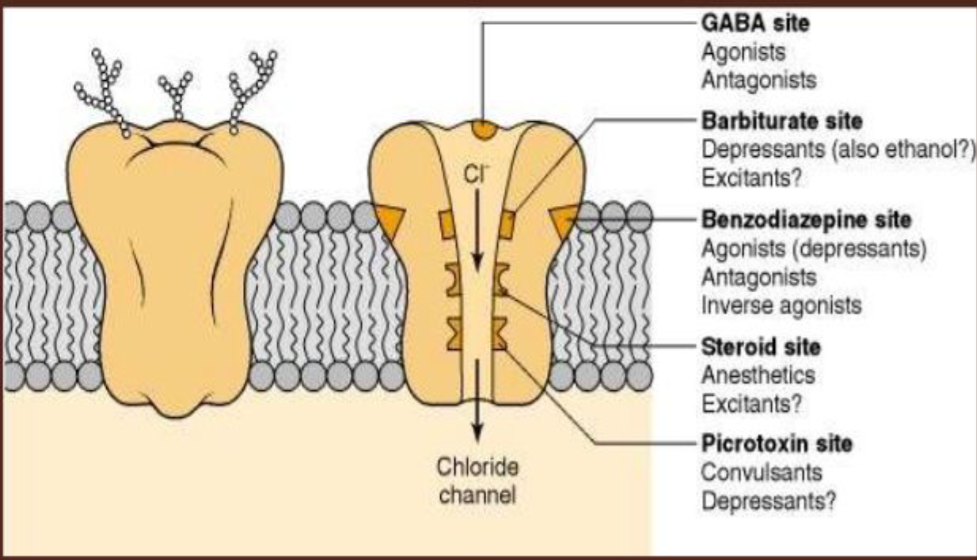
\includegraphics[width=0.6\textwidth, center]{images/image20.png}
    \caption{$\text{GABA}_A$ and its siote of actions.}
\end{figure}
The $\text{GABA}_A$ receptor is an ionotropic receptor and ligand-gated ion channel. 
Its endogenous ligand is $\gamma$-aminobutyric acid ($GABA$), the major inhibitory neurotransmitter in the central nervous system. 
Accurate regulation of GABAergic transmission through appropriate developmental processes, specificity to neural cell types, and responsiveness to activity is crucial for the proper functioning of nearly all aspects of the central nervous system (CNS).
Upon opening, the $\text{GABA}_A$ receptor on the postsynaptic cell is selectively permeable to chloride ions ($Cl^-$). 
\\
This receptor is the target of many drugs and active compounds:

\begin{itemize}
    \item \textbf{GABA site}
    \begin{itemize}
        \item Agonists: Mimic GABA and activate the receptor (e.g., muscimol\footnote{\textbf{Muscimol} (also known as agarin or pantherine) is the principal psychoactive constituent of Amanita muscaria and Amanita pantherina. Muscimol is a potent and selective orthosteric agonist for the GABAA receptor and displays sedative-hypnotic, depressant and hallucinogenic psychoactivity.}).
        \item Antagonists: Block GABA binding, inhibiting the receptor (e.g., bicuculline\footnote{\textbf{Bicuculline} is a phthalide-isoquinoline compound that is a light-sensitive competitive antagonist of GABAA receptors. It was originally identified in 1932 in plant alkaloid extracts. Since it blocks the inhibitory action of GABA receptors, the action of bicuculline mimics epilepsy; it also causes convulsions. This property is utilized in laboratories around the world in the in vitro study of epilepsy, generally in hippocampal or cortical neurons in prepared brain slices from rodents. \cite{bicuculline}}).
    \end{itemize}

    \item \textbf{Barbiturate site}
    \begin{itemize}
        \item Barbiturates\footnote{\textbf{Barbiturates} are a class of depressant drugs that are chemically derived from barbituric acid. They are effective when used medically as anxiolytics, hypnotics, and anticonvulsants, but have physical and psychological addiction potential as well as overdose potential among other possible adverse effects. Barbiturates have largely been replaced by benzodiazepines and nonbenzodiazepines ("Z-drugs") in routine medical practice, particularly in the treatment of anxiety disorders and insomnia, because of the significantly lower risk of overdose, and the lack of an antidote for barbiturate overdose. Despite this, barbiturates are still in use for various purposes: in general anesthesia, epilepsy, treatment of acute migraines or cluster headaches, acute tension headaches, euthanasia, capital punishment, and assisted suicide.} (e.g., phenobarbital): Bind here and enhance GABA action by prolonging the duration of chloride channel opening.
        \item May also be affected by ethanol.
        \item High doses can directly activate the receptor even in the absence of GABA.
    \end{itemize}

    \item \textbf{Benzodiazepine site}
    \begin{itemize}
        \item Agonists (e.g., diazepam, lorazepam): Potentiate GABA by increasing the frequency of channel opening.
        \item Antagonists (e.g., flumazenil): Block the site, reversing benzodiazepine effects.
        \item Inverse Agonists: Reduce GABAergic activity (may cause anxiety or seizures).
    \end{itemize}
\end{itemize}

\subsection{Antagonists}
Drugs that bind to its receptor and does not activate it, will prevent the action of an agonist.
The affinity is higher than the agonist and the efficacy is $0$.

\begin{figure}[H]
    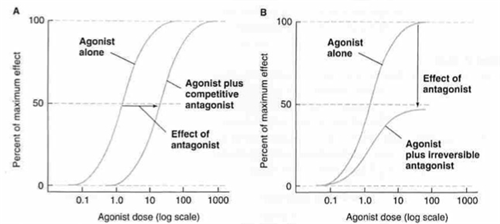
\includegraphics[width=0.7\textwidth, center]{images/image21.png}
    \caption{Characteristics of antagonists: \textbf{a) competitive}: shift agonist curve to the right. Resembles substrate [S], blocks active site but can be overcome by $\uparrow$ [S], $\downarrow$ potency, $\uparrow$ $K_m$ and $Vmax$ is unchanged. \textbf{b) non-competitive}: shift agonist curve downward. USUALLY Does not resemble [S], dose not block active site, therefore no $\uparrow$ [S] can overcome the effect, $\downarrow$ efficacy and potency, $\downarrow$ $Vmax$, and $Km$ is unchanged. $\uparrow$ EC50 of agonist (half maximally effective concentration for producing a given effect. \cite{bulltes})
}
\end{figure}

Antagonism can be:

\begin{itemize}
    \item \textbf{Competitive}
    \begin{itemize}
        \item The antagonism is reversible, agonist and antagonist compete for the same receptor.
        \item Antagonism can be overcome by increased concentration of agonist.
        \item When we plot the dose-response curve we see a parallel shifting.
    \end{itemize}

    \item \textbf{Non-Competitive}
    \begin{itemize}
        \item Irreverisble binding of receptor.
        \item Agonist cannot compete with antagonist.
        \item There will be resynthesis of the receptor and action will be regained.
    \end{itemize}
\end{itemize}
\textbf{Competitive} antagonists are sub-classified as reversible (\textbf{surmountable}) or irreversible (\textbf{insurmountable}) competitive antagonists, depending on how they interact with their receptor protein targets.
Reversible antagonists, which bind via noncovalent intermolecular forces, will eventually dissociate from the receptor, freeing the receptor to be bound again.
Irreversible antagonists bind via covalent intermolecular forces.
Because there is not enough free energy to break covalent bonds in the local environment, the bond is essentially "permanent", meaning the receptor-antagonist complex will never dissociate. 
The receptor will thereby remain permanently antagonized until it is ubiquitinated and thus destroyed.
\\
\\
\textbf{Non-competitive} antagonist is a type of insurmountable antagonist that may act in one of two ways: \textbf{by binding to an allosteric site of the receptor, or by irreversibly binding to the active site of the receptor}.
While the mechanism of antagonism is different in both of these phenomena, they are both called "non-competitive" because the end-results of each are functionally very similar. 
Unlike competitive antagonists, which affect the amount of agonist necessary to achieve a maximal response but do not affect the magnitude of that maximal response, non-competitive antagonists reduce the magnitude of the maximum response that can be attained by any amount of agonist.

\subsection{Allosteric Modulators}
Allosteric modulators affect the interaction of the receptor and the ligand by binding to separate
sites on the receptor. 
These effects are transmitted through changes in the receptor protein.

\begin{figure}[H]
    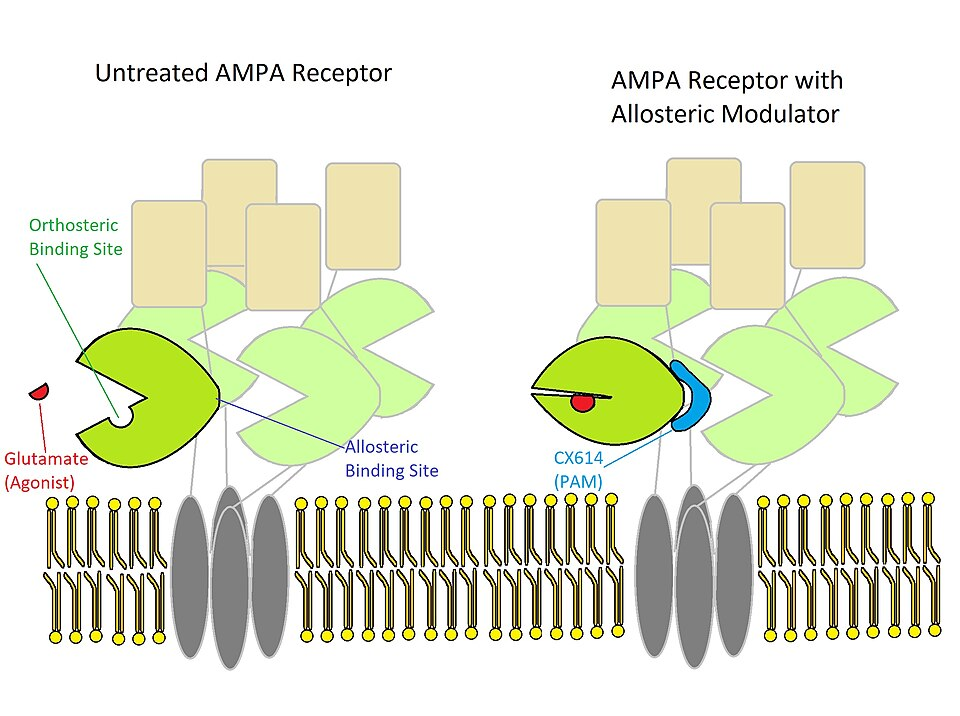
\includegraphics[width=0.6\textwidth, center]{images/image22.png}
    \caption{Some modulators act to stabilize conformational changes associated with the agonist-bound state. This increases the probability that the receptor will be in the active conformation, but does not prevent the receptor from switching back to the inactive state. With a higher probability of remaining in the active state, the receptor will bind agonist for longer. AMPA receptors modulated by aniracetam and CX614 will deactivate slower, and facilitate more overall cation transport. This is likely accomplished by aniracetam or CX614 binding to the back of the "clam shell" that contains the binding site for glutamate, stabilizing the closed conformation associated with activation of the AMPA receptor.}
\end{figure}

Allosteric modulators can be:

\begin{itemize}
    \item Positive allosteric modulators (PAMs) $\rightarrow$ enhance receptor activity.
    \item Negative allosteric modulators (NAMs) $\rightarrow$ reduce receptor activity (non-competitive inhibition).
    \item Silent allosteric modulators (SAMs) $\rightarrow$ bind but don’t modulate alone.
\end{itemize}

Important: All NAMs are non-competitive antagonists, but not all non-competitive antagonists are allosteric — some bind irreversibly to the orthosteric site (the main agonist site).

\begin{figure}[H]
    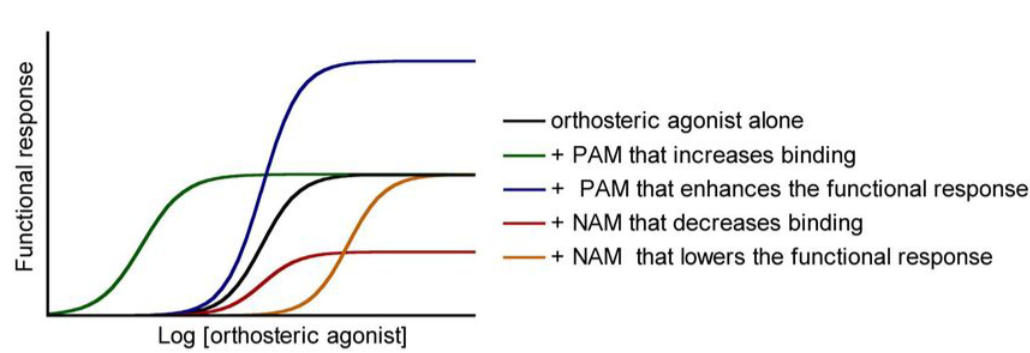
\includegraphics[width=0.7\textwidth, center]{images/image23.png}
    \caption{PAMs shift initial agonist response curve to lower agonist concentrations by increasing affinity and/or increase maximum response by increasing efficacy. NAMs shift curves to higher concentrations by decreasing affinities and/or lower maximum responses by decreasing efficacies. If compared to PAMs, the effects of NAMs are inverse.}
\end{figure}

\section{Take Home Message}

\begin{figure}[H]
    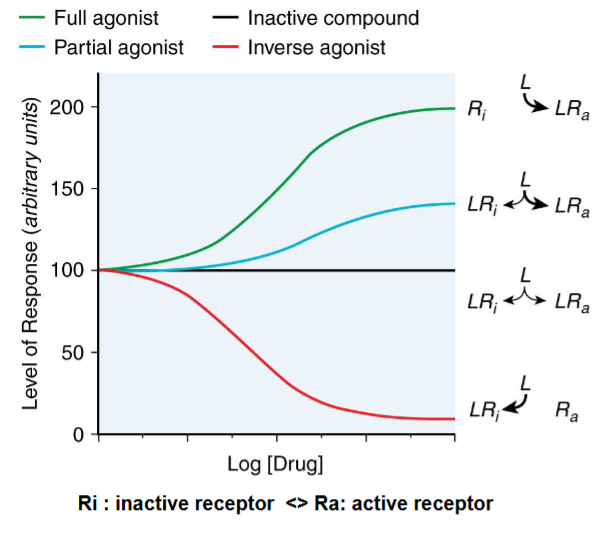
\includegraphics[width=0.7\textwidth, center]{images/image24.png}
\end{figure}

\chapter{Drugs: Addiction and Habituation}
\section{Tolerance}
Tolerance is the reduction of effect of a drug after its continuous adminsitration.
The body adapts to the chronic use of a substance and develop tolerance.
When looking at a dose-response plot, tolerance presents as

\begin{itemize}
    \item Decreased efficacy (downward shift),
    \item Decreased potency (rightward shift).
\end{itemize}

\begin{figure}[H]
   \centering
   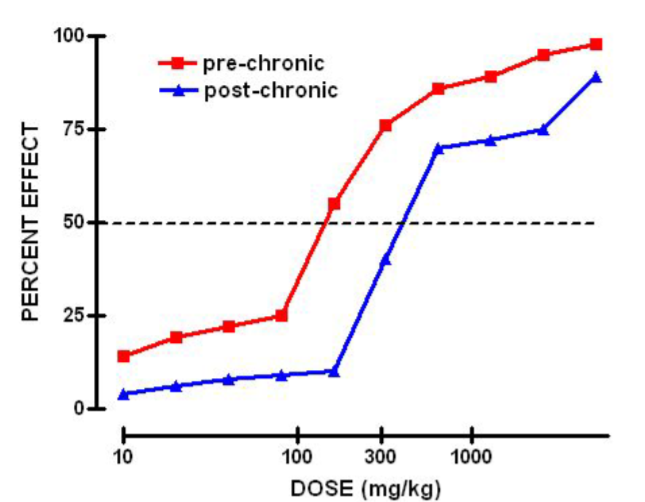
\includegraphics[width=0.5\textwidth]{images3/image.png}
\end{figure}

We can define three different types of "tolerance":
\begin{itemize}
    \item \textbf{Tachyphylaxis}: When desensitization occurs rapidly (Acute tolerance). E.g. amphetamines, that release a masive amount of dopamine.
    \item \textbf{Tolerance}: More gradual in responsiveness to drug (days or weeks)
    \item \textbf{Refractoriness/Drug resistance}: Loss of therapeutic efficacy (chemotherapy).
\end{itemize}

\subsection{Mechanisms of Tolerance}
\subsubsection{Metabolic (pharmacokinetic) Tolerance}
Importantly, we often refer to receptors when talking about tolerance, but can it can also involve metabolism. 
For example, \textbf{alcohol} metabolism involves ethanol $\rightarrow$ acetaldehyde through the enzyme alcohol dehydrogenase (ADH), and subsequently acetaldehyde $\rightarrow$ acetate through the enzyme
aldehyde dehydrogenase (ALDH). 
Chronic alcohol consumption can induce the microsomal ethanol oxidizing system (MEOS), particularly cytochrome P450 2E1 (CYP2E1).
This pathway becomes more active, increasing ethanol clearance from the body.
Result: Lower blood alcohol concentration (BAC) for the same dose $\rightarrow$ person feels less intoxicated.
Ultimately, ethanol becomes metabolized faster, contributing to \textbf{metabolic tolerance}.
Similarly, \textbf{amphetamines} alter renal filtrate pH, making it more acidic, which increases excretion of amphetamine.

\subsubsection{Physiological (pharmacodynamic, cellular) Tolerance}
\begin{itemize}
    \item e.g., receptor affinity or number altered by drug actions
    \item disruption of homeostatic processes may be critical
\end{itemize}

\subsubsection{Behavioral Tolerance}
\begin{itemize}
    \item Learning to compensate for drug-induced impairments
    \item respondent or operant conditioning
\end{itemize}

\section{GPCR}
G-protein-coupled receptors (GPCRs) are the largest and most diverse group of membrane receptors in eukaryotes (humans alone have nearly 1,000 different GPCRs, and each one is highly specific to a particular signal). 
These cell surface receptors act like an inbox for messages in the form of light energy, peptides, lipids, sugars, and proteins. 
Such messages inform cells about the presence or absence of life-sustaining light or nutrients in their environment, or they convey information sent by other cells.
\\
GPCRs play a role in an incredible array of functions in the human body, and increased understanding of these receptors has greatly affected modern medicine. 
In fact, researchers estimate that between one-third and one-half of all marketed drugs act by binding to GPCRs.
\\
\\
GPCRs consist of a single polypeptide that is folded into a globular shape and embedded in a cell's plasma membrane. 
Seven segments of this molecule span the entire width of the membrane — explaining why GPCRs are sometimes called seven-transmembrane receptors — and the intervening portions loop both inside and outside the cell. 
The extracellular loops form part of the pockets at which signaling molecules bind to the GPCR.
\\
\\
As their name implies, GPCRs interact with G proteins in the plasma membrane. 
When an external signaling molecule binds to a GPCR, it causes a conformational change in the GPCR. 
This change then triggers the interaction between the GPCR and a nearby G protein.

G proteins are specialized proteins with the ability to bind the nucleotides guanosine triphosphate (GTP) and guanosine diphosphate (GDP). 
Some G proteins, such as the signaling protein Ras, are small proteins with a single subunit. However, the G proteins that associate with GPCRs are heterotrimeric, meaning they have three different subunits: an alpha subunit, a beta subunit, and a gamma subunit. Two of these subunits — alpha and gamma — are attached to the plasma membrane by lipid anchors (Figure \ref{fig:GPCR}).

\begin{figure}
   \centering
   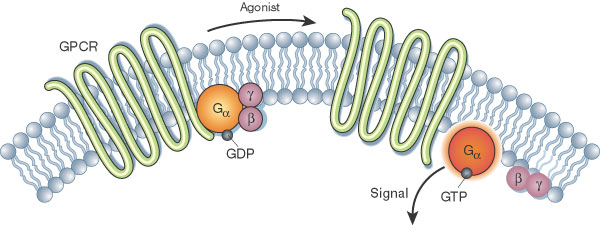
\includegraphics[width=0.7\textwidth]{images3/image2.png}
   \caption{\label{fig:GPCR} In unstimulated cells, the state of G alpha (orange circles) is defined by its interaction with GDP, G beta-gamma (purple circles), and a G-protein-coupled receptor (GPCR; light green loops). Upon receptor stimulation by a ligand called an agonist, the state of the receptor changes. G alpha dissociates from the receptor and G beta-gamma, and GTP is exchanged for the bound GDP, which leads to G alpha activation. G alpha then goes on to activate other molecules in the cell.}
\end{figure}

\subsection{GPCR desensitization}
While GPCR signaling is essential, overstimulation can be deleterious, resulting in cellular toxicity or uncontrolled cellular growth. 
Accordingly, nature has developed a number of mechanisms for limiting GPCR signaling, which are broadly referred to as desensitization, and refer to a decrease in response to repeated or continuous stimulation. 
We can distinguish two types of desensitization:

\begin{itemize}
    \item \textbf{Homologous desensitization}, in which the GPCR is downregulated;
    \item \textbf{Heterologous desensitization}, wherein the activated GPCR causes downregulation of a different GPCR. This downregulation is regulated by protein kinases-dependent phosphorylation of the intracellular (or cytoplasmatic) receptor domain.
\end{itemize}

Agonist binding also converts the receptor into a substrate for a family of kinases, the G-protein-couple receptor kinases (\textbf{GRKs}).
GRKs phosphorylate only agonist-activated receptors.
Subsequently, the phosphorylated receptor becomes a binding partner for \textbf{arrestins}.
Arrestins are normally cytosolic proteins, but they recognise agonist-activated, phosphorylated receptors and bind them. 
This binding makes the receptor inaccessible for G-proteins (i.e. the arrestin-bound receptor is desensitized), and it targets the receptor for internalization. 
This is because arrestins do not only bind receptors, but they also bind components of clathrin-coated pits.
Thus, arrestin-bound receptors move into clathrin-coated pits and are then ionternalized.
\\
\\
\textbf{Short-term desensitization} occurs over minutes, and is primarily associated with $\beta$-arrestins preventing G protein interaction with a GPCR. 
\textbf{Longer-term desensitization}, referred to as downregulation, occurs over hours to days, and involves receptor internalization into vesicles, degradation in lysosomes and decreased receptor mRNA levels through unclear mechanisms. 
Phosphorylation of the receptor by GPCR kinases (GRKs) and the recruitment of $\beta$-arrestins is critical to both these short- and long-term desensitization mechanisms. 
In addition to phosphorylation, both the GPCR and $\beta$-arrestins are modified post-translationally in several ways, including by ubiquitination. 
For many GPCRs, receptor ubiquitination promotes degradation of agonist-activated receptors in the lysosomes. 

\begin{figure}
   \centering
   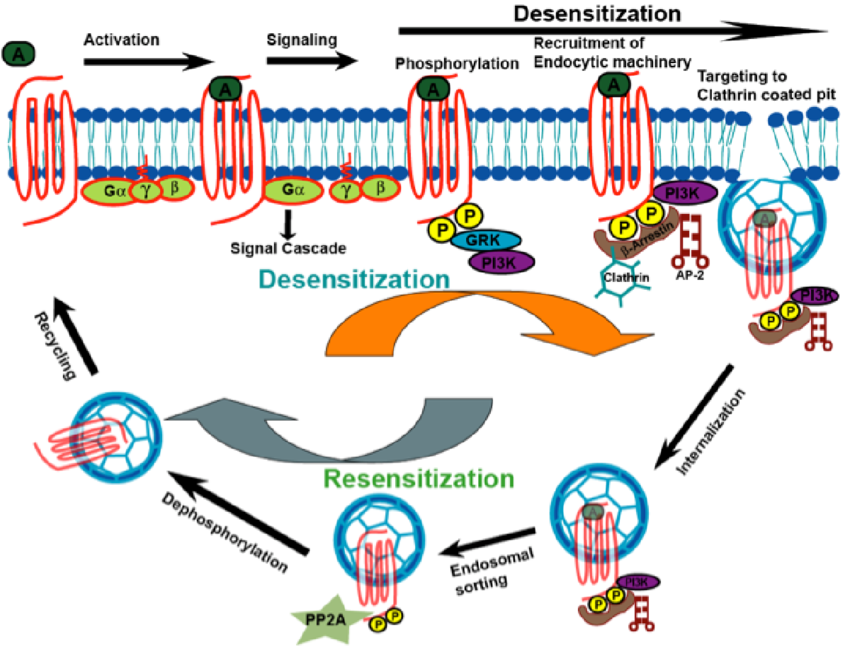
\includegraphics[width=0.7\textwidth]{images3/image3.png}
   \caption{\textbf{Classical view of desensitization, resensitization, and recycling of GPCRs}. When a ligand binds to the GPCR it causes a conformational change in the GPCR. The GPCR activates an associated G-protein by exchanging its bound GDP for a GTP. The G-protein's $\alpha$ subunit dissociates from the $\beta$ and $\gamma$ subunits to further affect intracellular signaling proteins or target functional proteins. The dissociated $\beta \gamma$ subunits facilitate the recruitment of GRK and PI3K to the receptor complex. The GRK phosphorylates C-terminal tail of the receptor which results in increased affinity and binding of the receptors to $\beta$-arrestins. Once bound, $\beta$-arrestins prevent G-protein coupling (desensitization) and may recruit other proteins AP-2 and clathrin required for receptor endocytosis (internalization). PI3K plays a role in generation of D3 phosphoinositides required for recruitment of AP-2 to the receptor complex. The membrane buds inwardly and pinched off from the membrane to form endocytic vesicles. Once internalized the receptors are trafficked to recycling endosomes or targeted to lysosomes for degradation. The receptors in the recycling endosomes are subsequently dephosphorylated by PP2A and recycled back to the plasma membrane as resensitized receptors.}
\end{figure}


\subsection{$\beta$-adrenergic receptors}
The adrenergic receptors or adrenoceptors are a class of GPCR that are targets of many catecholamines like norepinephrine (noradrenaline) and epinephrine (adrenaline) produced by the body, but also many medications like beta blockers, beta-2 ($\beta 2$) agonists and alpha-2 ($\alpha 2$) agonists, which are used to treat high blood pressure and asthma, for example.

\section{Nicotinic acetylcholine receptor}
Nicotinic acetylcholine receptors, or nAChRs, are receptor polypeptides that respond to the neurotransmitter \textbf{acetylcholine}. 
Nicotinic receptors also respond to drugs such as the agonist \textbf{nicotine}. 
They are found in the central and peripheral nervous system, muscle, and many other tissues of many organisms. 
At the neuromuscular junction they are the primary receptor in muscle for motor nerve-muscle communication that controls muscle contraction. 
In the peripheral nervous system: (1) they transmit outgoing signals from the presynaptic to the postsynaptic cells within the sympathetic and parasympathetic nervous system, and (2) they are the receptors found on skeletal muscle that receive acetylcholine released to signal for muscular contraction.

\begin{figure}%
    \centering
    \subfloat[\centering Nicotinic receptors are permeable to positive ions: Na+, K+ e Ca2+]{{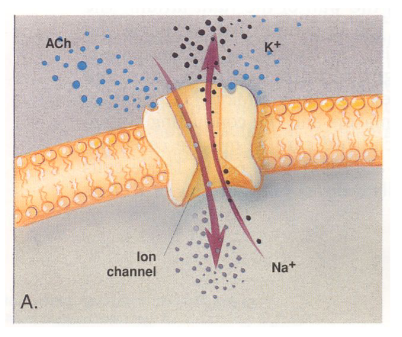
\includegraphics[width=0.3\textwidth]{images3/image4_1.png} }}%
    \qquad
    \subfloat[\centering Nicotinic receptors are found in the CNS and at the neuromuscular junction.]{{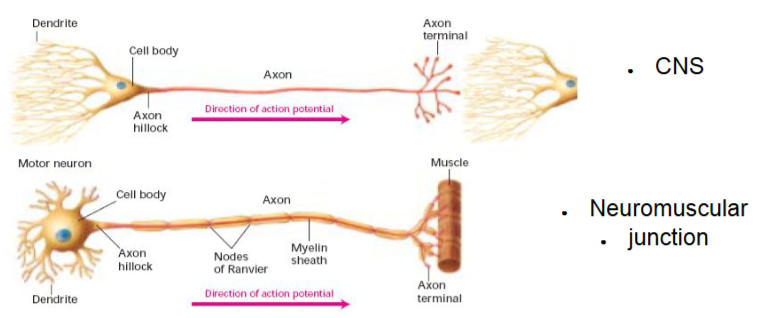
\includegraphics[width=0.6\textwidth]{images3/image4.png} }}%
    \caption{Nicotinic receptors}%
    \label{fig:example}%
\end{figure}

Common agonist drugs of the nicotinic receptor are \textbf{Succinylcholine}, used for muscle relaxation during anesthesia (it blocks the action of acetylcholine on skeletal muscles, depolarizing drug) and \textbf{carbachol}, used in ophtamology (it is a cholinomimetic drug that binds and activates acetylcholine receptors). 
An antagonist drug is \textbf{pancuronium}, that competitively inhibits the nicotinic acetylcholine receptor at the neuromuscular junction by blocking the binding of acetylcholine (non-depolarizing curare-mimetic muscle relaxant).

\subsection{Desensitization of nAChRs}
Nicotinic ACh receptors (nAChRs) can undergo desensitization, a reversible reduction in response during sustained agonist application.

\begin{figure}
    \centering
    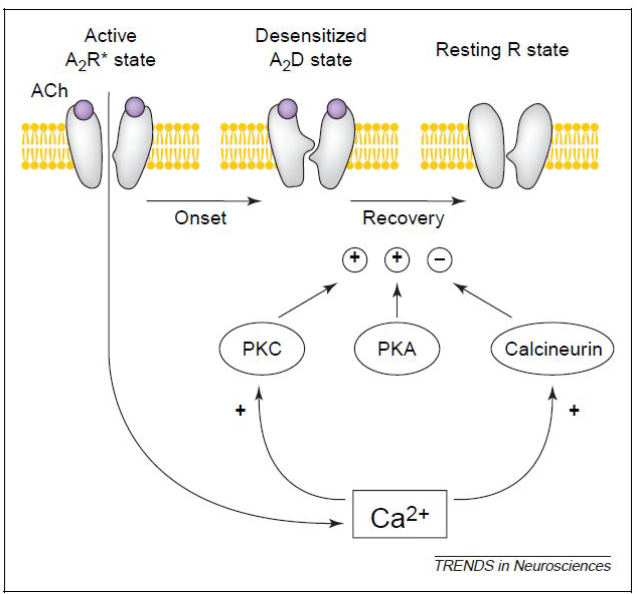
\includegraphics[width=0.4\textwidth]{images3/image5.png}
\end{figure}


In Figure \ref{fig:nic} it is depicted the rate of recovery from desensitization, measured by brief (i.e. 2 s) application of either 10 $\mu M$ nicotine or 100 $\mu M$ ACh, followed by a second application at the time intervals indicated (in seconds) above the responses. 
Note that after the ACh-induced desensitization, the peak amplitude of the test current returns to the control level (lower broken line) sooner than when nicotine is used to desensitize the receptors. 
Although nicotine (unlike ACh) can readily cross cell membranes and accumulate intracellularly, it is unlikely that the slow recovery rate from nicotine-evoked desensitization reflects the gradual release of this drug from a cell pool because the rate constant of nicotine uptake is $\approx 4 \times 10^{-3} min^{-1}$, thus largely in excess of the brief application time of nicotine shown here.
\\
When the onset and extent of desensitization are similar, the recovery of $\alpha 4 \beta 2$ receptors after the removal of nicotine requires much more time than recovery after the removal of ACh (agonist-dependent recovery.)
\\
\\
Take home message: when you smoke you should wait $1$ minute between puffs to really engage the nicotic receptors, otherwise they don't have time to recover.

\begin{figure}
    \centering
    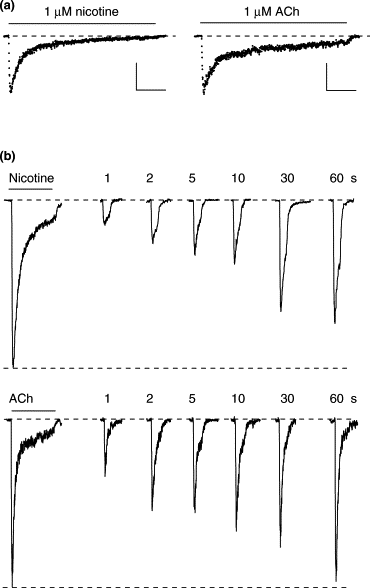
\includegraphics[width=0.4\textwidth]{images3/image6.png}
    \caption{\label{fig:nic}Differential onset and recovery from desensitization of $\alpha 4 \beta 2$ nAChRs activated by nicotine or ACh.}
\end{figure}


\section{Addiction}
\textbf{Addiction is defined as a chronic, relapsing brain disease that is characterized by compulsive drug seeking and use, despite harmful consequences}.
It is considered a brain disease because drugs change the brain - they change its structure and how it works. 
These brain changes can be long-lasting, and can lead to the harmful behaviors seen in people who abuse drugs.

A maladaptive pattern of substance use, leading to clinically significant impairment or distress, as manifested by three (or more) of the following, occurring at any time in the same 12 month period:

Tolerance
Withdrawal cryses
Substance taken in larger amounts or over a longer period than intended
Persistent desire or unsuccessful efforts to cut down or control substance use
Great deal of time spent in activities necessary to obtain substance, use substance
(e.g., chain smoking), or recover from effects
Important social, occupational, or recreational activities given up or reduced
because of substance use
Substance use continued despite knowledge of persistent or recurrent physical or
psychological problem likely to have been caused or exacerbated by substance





\printbibliography
\end{document}